\documentclass[11pt]{article}

\usepackage[a4paper]{geometry}
\usepackage{amssymb}
\usepackage{amsthm}
\usepackage{ngerman}
\usepackage{hyperref}
\usepackage{tikz}
\usepackage{csquotes}
\usepackage{fancyhdr}
\usepackage[T1]{fontenc}
\usepackage {enumerate}
\usepackage[utf8]{inputenc}
\usepackage{indentfirst}
\usepackage{algorithm}
\usepackage[noend]{algpseudocode}
\usepackage{lipsum}
\usepackage{amsmath}
\usepackage{mathtools}
\pagestyle{fancy}
\usetikzlibrary{automata}
\numberwithin{equation}{section}
\theoremstyle{definition}
\newtheorem*{env_definition}{Definition}
\theoremstyle{definition}
\newtheorem*{theorem} {Theorem}
\theoremstyle{definition}
\newtheorem*{env_satz}{Satz}
\theoremstyle{definition}
\newtheorem*{prop}{Behauptung}
\theoremstyle{definition}
\newtheorem*{bew}{Beweis}
\newcommand {\eps} {\varepsilon}
\algdef{SE}[SUBALG]{Indent}{EndIndent}{}{\algorithmicend\ }%
\algtext*{Indent}
\algtext*{EndIndent}

\title{Strassens Algorithmus für Matrixmultiplikation \\[3 mm] \large Ausarbeitung im Seminar \enquote{Algorithmen und Datenstrukturen} \\ am FG Theoretische Informatik / Formale Methoden \\ der Universit\"at Kassel}
\author{Bashar Khoulani}
\date{Wintersemester 2023/2024 \\ \phantom{a} \\ 13.02.2024}

\begin{document}
\maketitle

\begin{abstract}
Strassens Algorithmus ist ein rekursives Verfahren, das zwei Matrizen von der Ordnung $n \times n$ multipliziert und das Endergebnis liefert, wobei n $n \geq 1$ eine Zweierpotenz ist. 
Der Algorithmus ist auf das Prinzip der Divide-And-Conquer-Technik gestützt und seine asymptotische Laufzeit ist $\Theta(n^{\lg7})$.

Diese Seminararbeit befasst sich konkret mit dem Algorithmus von Strassen und liefert einen Vergleich zu den bekannten Verfahren für Matrixmultiplikation.
Dabei wird auf die Fragestellung eingegangen, wie Strassens Algorithmus für Matrixmultiplikation für die Nutzung in der Praxis geeignet ist.
\end{abstract}

\section{Einführung}\label{sec:einfuhrung}

Volker Strassen veröffentlichte seinen Algorithmus für Matrixmultiplikation in 1969\cite{Strassen1969}, der für eine große Aufmerksamkeit gesorgt hatte.
Davor galt das herkömmliche, naive Verfahren als die Norm.
Mit dem Algorithmus von Strassen wurde die Erkenntnis erworben, dass die Matrixmultiplikation in Hinsicht der asymptotischen Laufzeit subkubisch implementiert werden kann.
Viele Forscher haben sich seitdem damit befasst, noch schnellere Algorithmen für die Matrixmultiplikation zu entwickeln. 

Die Matrixmultiplikation übernimmt eine zentrale Rolle in zahlreichen Anwendungen,
wie beispielsweise in \ldots 
\begin{itemize}
    \item der Graphentheorie \cite{4569672},
    \item der Booleschen Algebra\cite{4569672, 1984},
    \item und in wichtigen Aspekten der linearen Algebra\cite{1984}.
\end{itemize}

Bevor Strassens Algorithmus vorgestellt wird, müssen vorher wichtige Grundlagen erläutert werden.
Dafür werden in Abschnitt~\ref{sec:abschn1} einige Themen aus dem Bereich der Algorithmen und Datenstrukturen erklärt und wiederholt.
Darüber hinaus werden das naive Verfahren, die Divide-And-Conquer-Variante und Strassens Algorithmus für die Matrixmultiplikation in Abschnitt~\ref{sec:abschn2} dargestellt.
Dazu werden die erwähnten Algorithmen in Hinsicht der asymptotischen Laufzeit analysiert und die Korrektheit von Strassens Algorithmus wird bewiesen.
In Abschnitt~\ref{sec:abschn3} werden die Algorithmen mithilfe vorgegebener Matrizen bewertet, um die Grenze einzusehen, wann Strassens Algorithmus günstiger als die herkömmlichen Varianten ist.
Zu guter Letzt werden die Ergebnisse in Abschnitt~\ref{sec:conclusion} zusammengefasst und es wird ein Ausblick in weiterführende Erkenntnisse bereitgestellt.
 
\section{Grundlagen}
\label{sec:abschn1}
Für die Bewertung und Analyse von Algorithmen haben sich viele Defintionen und Sätze in der Algorithmik und Mathematik verankert.
Um Strassens Algorithmus präzise zu bewerten, werden folgende Definitionen und Sätze aus der Vorlesung Algorithmen und Datenstrukturen zur Erfrischung wiederholt:
\begin{env_definition}[Landau-Symbole\cite{books/daglib/0023376}]
    Seien $f(n)$ und $g(n$) Funktionen.
    Dann werden folgende asymptotischen Schranken definiert:
    \begin{itemize}
        \item Obere Schranke:
        \[
            \mathcal{O}(g) = \{f\ |\,\exists\,c\,\in \mathbb{R}^{> 0}, n_0 \in \mathbb{N}^{> 0}\; \forall \,n \geq n_0: 0 \leq f(n) \leq c\,g(n)\}
        \]
        In anderen Worten: $\mathcal{O}(g)$ ist die Menge der Funktionen, die durch die Funktion $g$ nach oben beschränkt sind.
        \item Untere Schranke:
        \[
            \Omega(g) = \{f\ |\, \exists\,c\,\in \mathbb{R}^{> 0}, n_0 \in \mathbb{N}^{> 0}\; \forall n \geq n_0: 0 \leq c\,g(n) \leq f(n) \}
        \]
        Das bedeutet informell: $\Omega(g)$ ist die Menge der Funktionen, die durch die Funktion $g$ nach unten beschränkt sind.
        \item Scharfe Schranke:
        \[
            \Theta(g) = \{f\ |\, \exists\,c_1,\,c_2\,\in \mathbb{R}^{> 0}, n_0 \in \mathbb{N}^{> 0}\; \forall n \geq n_0: 0 \leq c_1\,g(n) \leq f(n) \leq c_2\,g(n)\}
        \]
        Das heißt: $\Theta(g)$ ist die Menge der Funktionen, die durch die Funktion $g$ mit positiven Konstanten $c_1$ und $c_2$ eingeschlossen sind.
        Es gilt außerdem:
        \[
            f \in \Theta(g) \iff f \in \Omega(g) \land f \in \mathcal{O}(g)
        \]
    \end{itemize}
\end{env_definition}

Mithilfe von Landau-Symbolen kann somit das asymptotische Verhalten von Funktionen bestimmt werden, das aus einem Algorithmus herausgeht.
Dieses signalisiert die Zeitkomplexität dieses Algorithmus und liefert eine Möglichkeit, diesen Algorithmus gegenüber anderen Algorithmen, die dasselbe Problem lösen, zu bewerten.
\newpage
Teile-und-Herrsche (Divide-and-Conquer) ist ein Design-Prinzip in der Algorithmik.
Algorithmen dieser Art verfolgen folgende Herangehensweise:
\begin{itemize}
    \item Löse kleine Instanzen unmittelbar
    \item Löse große Instanzen $I$ auf folgende Art und Weise:
    \begin{itemize}
        \item Teile die Instanz $I$ auf kleinere Instanzen $I_{1}$, $\dots$, $I_{k}$ (Divide)
        \item Löse die Instanzen $I_{1}$, $\dots$, $I_{k}$ (Conquer)
        \item Kombiniere die Lösungen der Instanzen $I_{1}$, $\dots$, $I_{k}$ zu einer Lösung für $I$
    \end{itemize}
\end{itemize}
Anhand der beschriebenen Herangehensweise ist ein rekursives Verfahren zu erkennen.
Weniger erkennbar bei rekursiven Algorithmen sind ihre Laufzeiten.
Somit werden üblicherweise ihre Rekurrenzgleichungen aufgestellt, die mittels des Master-Theorems meistens direkt ihre Laufzeiten liefern können.
\begin{theorem}[Master-Theorem]
    Seien $a \geq 1$ und $b > 1$ Konstanten.
    Sei $ f: \mathbb{R}^{\geq 0} \rightarrow \mathbb{R}^{\geq 0}$ eine Funktion, und sei $T : \mathbb{N} \rightarrow \mathbb{N}$ durch die folgende Rekursion definiert:
    \[
        T(n) = a \cdot T \left(\frac{n}{b}\right) + f(n)
    \]
    Dann gilt:
    \begin{enumerate}
        \item Wenn $f(n) \in \mathcal{O}(n^{log_b\;a-\eps}) $ für ein $\eps$ $>$ $0$, dann gilt $T(n) \in \Theta(n^{log_b\;a})$.
        \item Wenn $f(n) \in \Theta(n^{log_b\;a})$, dann gilt $T(n) \in \Theta(n^{log_b\;a}\;\lg\,n)$.
        \item Wenn $f(n) \in \Omega(n^{log_b\;a+\eps}) $ für ein $\eps$ $>$ $0$ und $a\,f\left(\frac{n}{b}\right) \leq c\,f(n)$ für ein $c$ $<$ $1$ und hinreichend großen n, dann gilt $T(n) \in \Theta(f(n))$.
    \end{enumerate}
\end{theorem}

Bei der Rekurrenzgleichung gibt das Parameter $a$ die Anzahl der rekursiven Aufrufe innerhalb des Algorithmus an, wobei das Parameter $b$ für den Reduzierungsfaktor von der Eingabe bei jedem rekursiven Aufruf steht. Die zusätzlichen Kosten, die neben den rekursiven Aufrufen im Algorithmus entstehen, werden durch $f(n)$ angegeben.

\bigskip
\textbf{Beispiel} Sei die folgende Rekurrenzgleichung gegeben:
\begin{equation}
    T(n) =
    8\; T\left(\frac{n}{2}\right) + f(n),\text{ mit }f(n) \in \Theta(n^{2})\label{eq:equation}
\end{equation}
Wir setzen $a = 8$, $b = 2$ und $f(n) \in \Theta(n^{2})$ und somit gilt $n^{log_b\;a} = n^{log_2\;8} = n^3$.
Mit $\eps = 1$ gilt der erste Fall, also $f(n) \in \mathcal{O}(n^{3-\eps})$, und es folgt $T(n) \in \Theta(n^{log_b\;a}) = \Theta(n^{log_2\;8}) = \Theta(n^{3})$.

\section{Matrixmultiplikation}
\label{sec:abschn2}
Die Matrixmultiplikation ist eine binäre Verknüpfung auf der Menge der Matrizen über den Ring $R$. Sie ist assoziativ, aber nicht kommutativ. Es gilt also $(AB)C = A(BC)$ und $AB \neq BA$ für $A \neq B$ \cite{Fischer2014}.
Sie ist über die folgende Abbildung definiert: 
\[
\cdot: R^{n\times l} \times R^{l\times m} \rightarrow R^{n\times m}, (A, B) \mapsto C = A \cdot B
\]
\[
c_{ij} = \sum_{k=1}^{l} a_{ik}b_{kj} \text{, für }i = 1, \dots, n \text{ und }j = 1, \dots, m
\]

Die einzelnen Einträge der Matrix $C$ können mithilfe der obigen Summenformel bestimmt werden. Im Folgenden wird angenommen, dass die Matrizen immer in quadratischer Form gegeben sind. Nach Definition der Matrixmultiplikation folgt dann, dass die Matrizen der gleichen Ordnung sind. 
\subsection{Naives Verfahren für die Matrixmultiplikation}
Der Algorithmus \ref{naiv} gibt das \enquote{naive} Verfahren an, das aus der Matrixmultiplikation hergeleitet werden kann. Angenommen haben die Matrizen das Attribut $zeilen$, welches die Anzahl der Zeilen der Matrix angibt, dann stellen wir fest:
Angenommen sind die Matrizen quadratisch, dann berechnet die erste \textbf{for}-Schleife die Einträge von der Matrixzeile $i$ und mit der Matrixzeile $i$ berechnet die zweite \textbf{for}-Schleife in der Spalte $j$ den Eintrag $c_{ij}$. Dabei wird die vorige Summenformel verwendet, um den Eintrag zu bestimmen. Die innerste \textbf{for}-Schleife entspricht also der Summenformel. Daraus erschließt sich wegen der Form der \textbf{for}-Schleifen, mit jeweils $n$ Iterationen, eine Laufzeit von $\Theta(n^3)$, wobei n für die Anzahl der Zeilen steht. 
\begin{algorithm}[hbt!]
\begin{algorithmic}[1]
\caption{MATRIX-MULT - NAIV}
\label{naiv}
\Procedure{MATRIX-MULT}{$A,B$}
    \State $n\gets A.zeilen$
    \State $C$ sei eine neue $n\times n$-Matrix
    \For{$i \gets 1$ $bis$ $n$}
        \For{$j \gets 1$ $bis$ $n$}
            \State $c_{ij} \gets 0$
            \For{$k \gets 1$ $bis$ $n$}
                \State {$c_{ij}$ $\gets$ {$c_{ij} + a_{ik} \cdot b_{kj}$}}
            \EndFor
        \EndFor
    \EndFor
    \State \textbf{return} $C$ 
\EndProcedure
\end{algorithmic}
\end{algorithm}

\subsection{Divide-And-Conquer Verfahren}

Neben dem \enquote{naiven} Verfahren kann ein rekursives Verfahren aufgestellt werden, das die Divide-And-Conquer Technik benutzt. Dabei wird angenommen, dass die Matrizen quadratisch sind und eine Größenordnung von einer Zweierpotenz haben. Dies ist nötig, um die Matrizen (große Instanzen) in jedem rekursiven Aufruf in Teilmatrizen (kleine Instanzen) von der Dimension der Zeilen bzw. Spalten zu halbieren. 

Der Algorithmus \ref{dac} gibt das Divide-And-Conquer Verfahren an. Beim Basisfall auf unterster Ebene mit $n = 1$ ist eine Skalarmultiplikation durchzuführen. Sonst werden die Matrizen in vier Teilmatrizen aufgeteilt. Dann werden die Teilmatrizen auf analoge Weise wie beim \enquote{naiven} Verfahren als Elemente betrachtet, um die Matrixmultiplikation durchzuführen. Dies passiert von Zeile 19 bis Zeile 22. Nach Abschluss aller rekursiven Aufrufe und dem Zusammenführen der Teilmatrizen wird das Produkt in Zeile 23 zurückgegeben.

\begin{algorithm}[hbt!]
\begin{algorithmic}[1]
\caption{MATRIX-MULT-DAC - DIVIDE-AND-CONQUER}
\label{dac}
\Procedure{MATRIX-MULT-DAC}{$A,B$}
    \State $n\gets A.zeilen$
    \If {$n$ $==$ $1$}
        \State $c_{11}\gets a_{11}\cdot b_{11}$
    \Else  
        \State Seien $A$, $B$ und $C$ $n \times n$-Matrizen
        \State $A_{11}\gets A[1\dotsb n/2][1\dotsb n/2]$
        \State $B_{11}\gets B[1\dotsb n/2][1\dotsb n/2]$
        \State $C_{11}\gets C[1\dotsb n/2][1\dotsb n/2]$
        \State $A_{12}\gets A[1\dotsb n/2][n/2 + 1\dotsb n]$
        \State $B_{12}\gets B[1\dotsb n/2][n/2 + 1\dotsb n]$
        \State $C_{12}\gets C[1\dotsb n/2][n/2 + 1\dotsb n]$
        \State $A_{21}\gets A[n/2 + 1\dotsb n][1\dotsb n/2]$
        \State $B_{21}\gets B[n/2 + 1\dotsb n][1\dotsb n/2]$
        \State $C_{21}\gets C[n/2 + 1\dotsb n][1\dotsb n/2]$
        \State $A_{22}\gets A[n/2 + 1\dotsb n][n/2 + 1\dotsb n]$
        \State $B_{22}\gets B[n/2 + 1\dotsb n][n/2 + 1\dotsb n]$
        \State $C_{22}\gets C[n/2 + 1\dotsb n][n/2 + 1\dotsb n]$
        \State $C_{11}\gets \Call{MATRIX-MULT-DAC}{A_{11}, B_{11}}$ \newline
        \hspace*{4.65em} $+$ $\Call{MATRIX-MULT-DAC}{A_{12}, B_{21}}$
        \State $C_{12}\gets \Call{MATRIX-MULT-DAC}{A_{11}, B_{12}}$ \newline
        \hspace*{4.65em} $+$ $\Call{MATRIX-MULT-DAC}{A_{12}, B_{22}}$ 
        \State $C_{21}\gets \Call{MATRIX-MULT-DAC}{A_{21}, B_{11}}$ \newline
        \hspace*{4.65em} $+$ $\Call{MATRIX-MULT-DAC}{A_{22}, B_{21}}$
        \State $C_{22}\gets \Call{MATRIX-MULT-DAC}{A_{21}, B_{12}}$ \newline
        \hspace*{4.65em} $+$ $\Call{MATRIX-MULT-DAC}{A_{22}, B_{22}}$
    \EndIf
    \State \textbf{return} $C$ 
\EndProcedure
\end{algorithmic}
\end{algorithm}

Um den Algorithmus auf seine Laufzeit zu analysieren, wird die Rekurrenzgleichung aufgestellt. Dazu zählen wir die rekursiven Aufrufe -- im Algorithmus \ref{dac} sind das acht -- und extrahieren den Reduzierungsfaktor von der Eingabe -- im Algorithmus \ref{dac} ist der Faktor $2$. Die zusätzlichen Kosten enstehen durch die Matrixaddition, die in $\Theta(n^2)$ läuft. Die Partitionierung der Matrizen erfolgt konstant, da hier Indexberechnungen durchgeführt werden. Somit erhalten wir die Gleichung für $n > 1$, die in \ref{eq:equation} angegeben ist. Nach dem Anwenden des Master-Theorems stellen wir fest, dass der Divide-And-Conquer Algorithmus in derselben Laufzeitklasse wie das \enquote{naive} Verfahren liegt.

\subsection{Strassens Algorithmus}
Strassens rekursiver Algorithmus is keineswegs einleuchtend. Der Grundgedanke war es, die Anzahl der Matrixmultiplikationen zu reduzieren, um den Faktor $a$ -- die Anzahl der rekursiven Aufrufe innerhalb eines rekursiven Algorithmus -- bei der Anwendung des Master-Theorems zu verringern. 

Der Algorithmus beruht auf eine Intuition, die mittels der folgenden Gleichungen veranschaulicht werden kann. Seien $x$, $y$ $\in \mathbb{R}$, dann gilt: $x^2 - y^2 \stackrel{1}{=} x \cdot x - y \cdot y \stackrel{2}{=} (x + y)(x - y)$. Die Gleichheit gilt bei Gleichung 1 soweiso, dabei ist die Anzahl der Multiplikationen und Additionen bzw. Subtraktionen gleich. Die Gleichheit gilt bei Gleichung 2 nach der dritten binomischen Formel. Somit sind aus zwei Produkten und einer Addition ein Produkt, eine Addition und eine Subtraktion entstanden. 

Angenommen sind die Matrizen quadratisch und haben eine Größenordnung von einer Zweierpotenz haben, dann berechnet das Verfahren \ref{strassen} die Matrixmultiplikation von $A$ und $B$ (Korrektheitsbeweis später). Im Ausblick wird der Fall für allgemeine Matrizen behandelt. Bei dem Algorithmus wird wieder auf unterster Ebene ($n = 1$) eine Skalarmultiplikation durchgeführt. Sonst werden die Matrizen in vier Teilmatrizen aufgeteilt. Dann greift in den Zeilen 19-39 der Kernpunkt von Strassens Algorithmus ein. Dabei werden folgende Produkte berechnet und die Matrix $C$ gesetzt:
\begin{align*} 
        P_{1} = A_{11} \cdot \left(B_{12} - B_{22}\right) \; \; \; \; & P_{2} = B_{22} \cdot \left(A_{11} + A_{12}\right) \\
        P_{3} = B_{11} \cdot \left(A_{21} + A_{22}\right) \; \; \; \; & P_{4} = A_{22} \cdot \left(B_{21} - B_{11}\right) \\
        P_{5} = \left(B_{11} + B_{22}\right) \cdot \left(A_{11} + A_{22}\right) \; \; \; \; & P_{6} = \left(B_{21} + B_{22}\right) \cdot \left(A_{12} - A_{22}\right) \\
        P_{7} = \left(A_{11} - A_{21}\right) \cdot \left(B_{11} + B_{12}\right) \; \; \; \; &
\end{align*}
\begin{equation}\label{eqstrassem}
    C =\left(\begin{array}{cc}
                P_{4} + P_{5} + P_{6} - P_{2} & P_{1} + P_{2} \\
                P_{3} + P_{4} & P_{1} + P_{5} - P_{3} - P_{7} 
            \end{array}\right)
\end{equation}

Wir haben also die acht Produkte von der Divide-And-Conquer-Variante auf sieben Produkte reduziert. Dennoch haben wir aber nun 18 Additionen und Subtraktionen, anstatt von vier. 

Wir führen den Korrektheitsbeweis folgendermaßen durch: Die einzelnen Einträge der Matrix $C$ werden auf die Gleichungen aus dem Divide-And-Conquer Algorithmus \ref{dac} zusammengefasst. Somit wird eine Äquivalenz zwischen Strassens Algorithmus und dem Divide-And-Conquer Algorithmus hergestellt. Die Äquivalenz zwischen dem Divide-And-Conquer Algorithmus und dem \enquote{naiven} Verfahren besteht auf intuitive Weise bereits. Auf diese Art und Weise erhalten wir eine Äquivalenz zwischen den drei Algorithmen. O. B. d. A. werden die Matrixdimensionen als Zweierpotenzen vorausgesetzt. Es liegt nun folgende Behauptung vor:

\begin{prop}
    $A \cdot B = C$
\end{prop}

\begin{bew}
    Seien $A$, $B$ und $C$ $\in R^{n \times n}$, wobei $n \geq 2$ eine Zweierpotenz ist. Wir teilen die Matrizen in vier Blöcke auf, wie in Algorithmus \ref{strassen} in Zeile 7-18. Dann gilt gemäß \ref{eqstrassem}:
    \begin{equation*}
        \begin{multlined}
            C_{11} = P_{4} + P_{5} + P_{6} - P_{2} = \\
            \arraycolsep=1.4pt
            \begin{array}{ccccccc}
                A_{11} \cdot B_{11} & + A_{11} \cdot B_{22} & + A_{22} \cdot B_{11} & + A_{22} \cdot B_{22} &&& \\
                && - A_{22} \cdot B_{11} && + A_{22} \cdot B_{21}&& \\
                & - A_{11} \cdot B_{22} &&&& - A_{12} \cdot B_{22}& \\
                &&& - A_{22} \cdot B_{22} & - A_{22} \cdot B_{21} & + A_{12} \cdot B_{22} & + A_{12} \cdot B_{21} \\
            \end{array} \\
            = A_{11} \cdot B_{11} + A_{12} \cdot B_{21}
        \end{multlined}
    \end{equation*}
    Somit erhalten wir die Gleichung von $C_{11}$ aus dem Algorithmus \ref{dac}.
    
    \begin{equation*}
        \begin{multlined}
            C_{12} = P_{1} + P_{2} = \\
            \arraycolsep=1.4pt
            \begin{array}{ccc}
                A_{11} \cdot B_{12} & - A_{11} \cdot B_{22} &\\
                & + A_{11} \cdot B_{22} & + A_{12} \cdot B_{22} \\
            \end{array} \\
            = A_{11} \cdot B_{12} + A_{12} \cdot B_{22}
        \end{multlined}
    \end{equation*}
    Dies entspricht der Gleichung von $C_{12}$ aus dem Algorithmus \ref{dac}.
    
    \begin{equation*}
        \begin{multlined}
            C_{21} = P_{3} + P_{4} = \\
            \arraycolsep=1.4pt
            \begin{array}{ccc}
                A_{21} \cdot B_{11} & + A_{22} \cdot B_{11} &  \\
                & - A_{22} \cdot B_{11} & + A_{22} \cdot B_{21} \\
            \end{array} \\
            = A_{21} \cdot B_{11} + A_{22} \cdot B_{21}
        \end{multlined}
    \end{equation*}
    Es folgt, dass dies der Gleichung von $C_{21}$ aus dem Algorithmus \ref{dac} entspricht.
    
    \begin{equation*}
        \begin{multlined}
            C_{22} = P_{1} + P_{5} - P_{3} - P_{7} = \\
            \arraycolsep=1.4pt
            \begin{array}{ccccccc}
                A_{11} \cdot B_{11} & + A_{11} \cdot B_{22} & + A_{22} \cdot B_{11} & + A_{22} \cdot B_{22} &&& \\
                & - A_{11} \cdot B_{22} &&& + A_{11} \cdot B_{12}&& \\
                && - A_{22} \cdot B_{11} &&& - A_{21} \cdot B_{11}& \\
                - A_{11} \cdot B_{11} &&&& - A_{11} \cdot B_{12} & + A_{21} \cdot B_{11} & + A_{21} \cdot B_{12} \\
            \end{array} \\
            = A_{21} \cdot B_{12} + A_{22} \cdot B_{22}
        \end{multlined}
    \end{equation*}
    Somit erhalten wir die Gleichung von $C_{22}$ aus dem Algorithmus \ref{dac}. Insgesamt erhalten wir dieselben Gleichungen aus dem Divide-And-Conquer Algorithmus \ref{dac} für das Produkt $A \cdot B$. Somit gilt $A \cdot B = C$ und wir erhalten die Äquivalenz zwischen allen drei Algorithmen. \qed
\end{bew}

Wir können aus dem Algorithmus \ref{strassen} die folgende Rekurrenzgleichung aufstellen: 
\[ T(n) =  \begin{cases*}
                    \Theta(1) & \text{n $\leq$ 1,} \\
                    7 \cdot T\left(\frac{n}{2}\right) + \Theta(n^2) & \text{n > 1} 
                \end{cases*}
\]
Wir wenden nun das Master-Theorem an: Wir setzen $a = 7$, $b = 2$ und $f(n) \in \Theta(n^{2})$ und somit gilt $n^{log_b\;a} = n^{log_2\;7}$.
Mit $\eps = 0,8$ ($2,80 < lg\;7 < 2,81$) gilt der erste Fall, also $f(n) \in \mathcal{O}(n^{3-\eps})$, und es folgt $T(n) \in \Theta(n^{log_b\;a}) = \Theta(n^{log_2\;7}) = \Theta(n^{lg\;7})$. Somit haben wir bzgl. der asymptotischen Analyse eine Verbesserung von $\Theta(n^{3})$ auf $\Theta(n^{lg\;7})$.
\begin{algorithm}[hbt!]
\begin{algorithmic}[1]
\caption{MATRIX-MULT-STRASSEN - STRASSEN}
\label{strassen}
\Procedure{MATRIX-MULT-STRASSEN}{$A,B$}
    \State $n\gets A.zeilen$
    \If {$n$ $==$ $1$}
        \State $c_{11}\gets a_{11}\cdot b_{11}$
    \Else  
        \State Seien $A$, $B$ und $C$ $n \times n$-Matrizen
        \State $A_{11}\gets A[1\dotsb n/2][1\dotsb n/2]$
        \State $B_{11}\gets B[1\dotsb n/2][1\dotsb n/2]$
        \State $C_{11}\gets C[1\dotsb n/2][1\dotsb n/2]$
        \State $A_{12}\gets A[1\dotsb n/2][n/2 + 1\dotsb n]$
        \State $B_{12}\gets B[1\dotsb n/2][n/2 + 1\dotsb n]$
        \State $C_{12}\gets C[1\dotsb n/2][n/2 + 1\dotsb n]$
        \State $A_{21}\gets A[n/2 + 1\dotsb n][1\dotsb n/2]$
        \State $B_{21}\gets B[n/2 + 1\dotsb n][1\dotsb n/2]$
        \State $C_{21}\gets C[n/2 + 1\dotsb n][1\dotsb n/2]$
        \State $A_{22}\gets A[n/2 + 1\dotsb n][n/2 + 1\dotsb n]$
        \State $B_{22}\gets B[n/2 + 1\dotsb n][n/2 + 1\dotsb n]$
        \State $C_{22}\gets C[n/2 + 1\dotsb n][n/2 + 1\dotsb n]$
        \State $S_{1}\gets A_{11} + A_{12}$
        \State $S_{2}\gets A_{11} + A_{22}$
        \State $S_{3}\gets A_{21} + A_{22}$
        \State $S_{4}\gets A_{11} - A_{21}$
        \State $S_{5}\gets A_{12} - A_{22}$
        \State $S_{6}\gets B_{11} + B_{12}$
        \State $S_{7}\gets B_{11} + B_{22}$
        \State $S_{8}\gets B_{21} + B_{22}$
        \State $S_{9}\gets B_{12} - B_{22}$
        \State $S_{10}\gets B_{21} - B_{11}$
        \State $P_1\gets \Call{MATRIX-MULT-STRASSEN}{A_{11}, S_{9}}$ 
        \State $P_2\gets \Call{MATRIX-MULT-STRASSEN}{S_{1}, B_{22}}$
        \State $P_3\gets \Call{MATRIX-MULT-STRASSEN}{S_{3}, B_{11}}$
        \State $P_4\gets \Call{MATRIX-MULT-STRASSEN}{A_{22}, S_{10}}$
        \State $P_5\gets \Call{MATRIX-MULT-STRASSEN}{S_{2}, S_{7}}$
        \State $P_6\gets \Call{MATRIX-MULT-STRASSEN}{S_{5}, S_{8}}$
        \State $P_7\gets \Call{MATRIX-MULT-STRASSEN}{S_{4}, S_{6}}$
        \State $C_{11}\gets P_{4} + P_{5} + P_{6} - P_{2}$
        \State $C_{12}\gets P_{1} + P_{2}$
        \State $C_{21}\gets P_{3} + P_{4}$
        \State $C_{22}\gets P_{1} + P_{5} - P_{3} - P_{7}$
    \EndIf
    \State \textbf{return} $C$ 
\EndProcedure
\end{algorithmic}
\end{algorithm}
\section{Bewertung}
\label{sec:abschn3}
Wir haben erfahren, dass Strassens Algorithmus in $\Theta(n^{lg\;7})$ läuft, wobei n für
die Anzahl der Zeilen eine Matrix steht. Somit soll der Algorithmus in der Praxis schneller als die zwei anderen Algorithmen laufen. Mit einer Implementierung in der Programmiersprache Java werden die drei Algorithmen auf verschiedene Matrixgrößen angewendet und getestet. Die Matrizen werden zufällig generiert und in den jeweiligen Algorithmus eingegeben. 

In Abbildung \ref{1} ist die Laufzeit in benötigten Zeiteinheiten pro Matrixgröße abgebildet. Eine Unstimmigkeit wird direkt festgestellt; Strassens Algorithmus ist langsamer als das \enquote{naive} Verfahren. Die Ursache liegt in der rekursiven Implementierung. In einer ersten Variante wird der Basisfall auf $n = 1$ gesetzt und somit werden die Matrizen soweit aufgeteilt, bis der Basisfall erreicht wird. Dadurch entsteht ein Rekursionsstack mit hoher Größe, deren Verwaltung viele Ressourcen verbraucht.

\begin{figure}[H]
    \center
    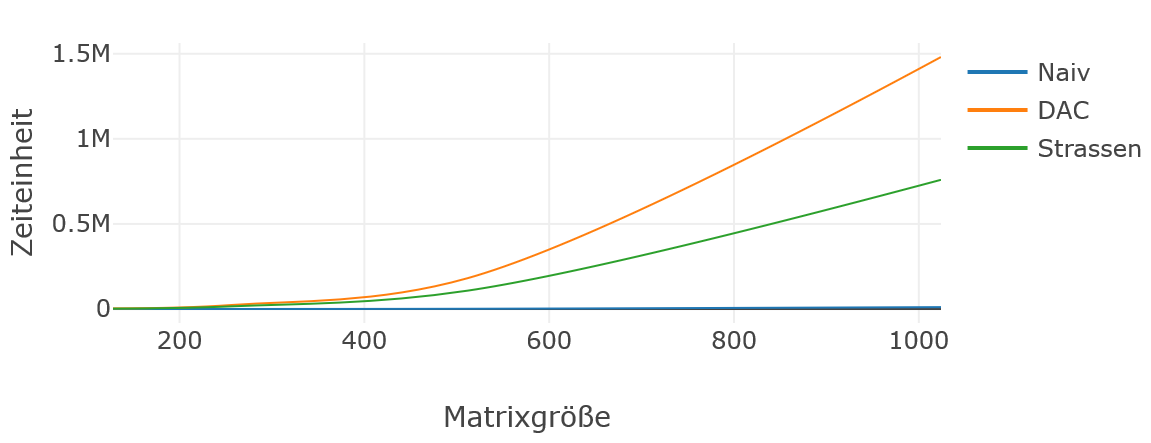
\includegraphics[scale=0.38]{basisfallnot.png}
    \caption{Basisfall $n = 1$}
    \label{1}
\end{figure}

Beim Setzen des Basisfalls auf $n = 32$ ist eine klare Verbesserung in Abbildung \ref{32} zu sehen. Auf diese Weise werden die Matrizen $A$ und $B$ ab einer bestimmten Größe ($n = 32$) mit dem \enquote{naiven} Verfahren multipliziert, sodass die Matrizen nicht in viele kleinen Teilmatrizen aufgeteilt werden. Daher ist für die praktische Anwendung von Strassens Algorithmus einen geeigneten \enquote{Crossover}-Punkt für den Basisfall zu wählen.
\begin{figure}[H]
    \center
    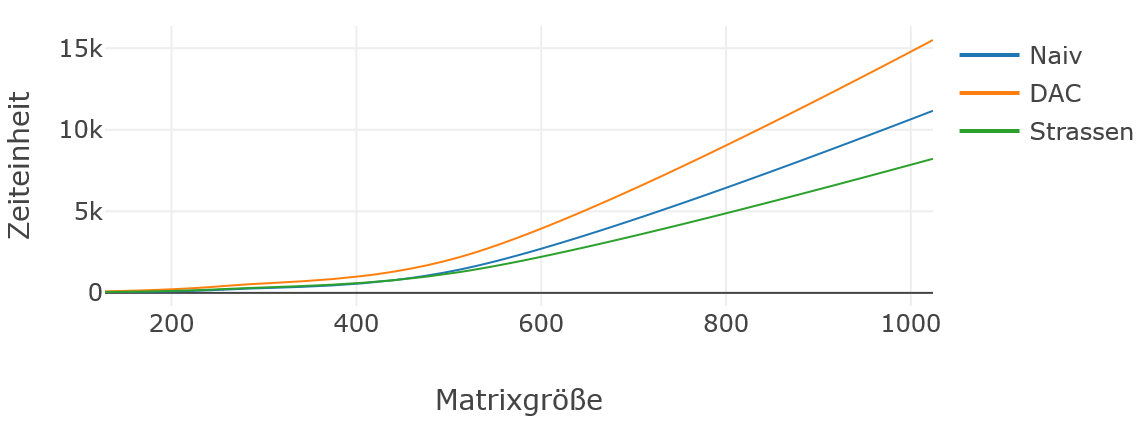
\includegraphics[scale=0.38]{basisfallmod.png}
    \caption{Basisfall $n = 32$}
    \label{32}
\end{figure}
\section{Ausblick und Zusammenfassung}
\label{sec:conclusion}

Es wurde festgestellt, dass Strassens Algorithmus in einer besseren asymptotischen Laufzeitklasse als der \enquote{naive} Algorithmus und der Divide-And-Conquer Algorithmus liegt. In der Praxis wird der Algorithmus jedoch leicht modifizert, also der Basisfall wird geändert, um den hohen Aufwand bei der Verwaltung des Rekursionsstack zu vermeiden. Strassens Algorithmus kann auch parallelisiert werden. Dabei werden die sieben Produkte aus Algorithmus \ref{strassen} gleichzeitig berechnet, was den Algorithmus verschnellert.

Um Strassens Algorithmus auf beliebige Matrixgrößen anwenden zu können, muss auch der Algorithmus modifizert werden. Dabei muss vor Anwendung des Algorithmus geprüft werden, ob die Eingabematrizen eine Zweierpotenz Größenordnung haben. Falls ja, dann wird der Algorithmus standardmäßig durchgeführt. Sonst werden die Matrizen auf eine Zweierpotenz Größenordnung vergrößert, indem zusätzliche, mit Null befüllte Spalten und Zeilen zu den Eingabematrizen hinzugefügt werden, bis sie eine Zweierpotenz Form haben. Bei dem Endprodukt werden dann die hinzugefügten Spalten und Zeilen entfernt.

Es existiert aktuell ein besserer Algorithmus hinsichtlich der asymptotischen Laufzeit als Strassens Algorithmus, nämlich der Coppersmith-Winograd Algorithmus, der in $\mathcal{O}(n^{2,376})$ läuft \cite{books/daglib/0023376}. Dieser Algorithmus ist dennoch in der Praxis eher unpraktisch und nur für Matrizen mit sehr hohen Größenordnungen gedacht. Jedoch ist er für die Theorie von bedeutsamer Wichtigkeit, um die theoretischen Grenzen der Zeitkomplexität der Matrixmultiplikation zu definieren.

Zu guter Letzt ist auch erwähnenswert, dass ein rekursiver Algorithmus für die Matrixmultiplikation von Matrizen mit einer Zweierpotenz Größenordnung mit weniger als sieben Produkte nicht existiert \cite{https://doi.org/10.48550/arxiv.math/0407224}. Somit ist Strassens Algorithmus der beste in dieser Hinsicht.

\newpage
\bibliographystyle{plain}
\bibliography{sem.bib}
\end{document}